%%
%% This is file `sample-sigconf.tex',
%% generated with the docstrip utility.
%%
%% The original source files were:
%%
%% samples.dtx  (with options: `sigconf')
%% 
%% IMPORTANT NOTICE:
%% 
%% For the copyright see the source file.
%% 
%% Any modified versions of this file must be renamed
%% with new filenames distinct from sample-sigconf.tex.
%% 
%% For distribution of the original source see the terms
%% for copying and modification in the file samples.dtx.
%% 
%% This generated file may be distributed as long as the
%% original source files, as listed above, are part of the
%% same distribution. (The sources need not necessarily be
%% in the same archive or directory.)
%%
%% The first command in your LaTeX source must be the \documentclass command.
\documentclass[sigconf]{acmart}

% TODO remove XD
\usepackage{xcolor}
\newcommand{\secfunc}[1]{{\color{magenta}#1}}
\newcommand{\mention}[1]{{\color{cyan}#1}}
\newcommand{\plan}[1]{{\color{purple}#1}}
\newcommand{\bp}[1]{{\color{violet}#1}}
\newcommand{\draft}[1]{{\color{blue}#1}}
\newcommand{\review}[1]{{\color{black}#1}}
\newcommand{\todo}[1]{{\color{orange}(#1)}}

\usepackage{listings}
\usepackage{tabularx}

%%
%% \BibTeX command to typeset BibTeX logo in the docs
\AtBeginDocument{%
  \providecommand\BibTeX{{%
    \normalfont B\kern-0.5em{\scshape i\kern-0.25em b}\kern-0.8em\TeX}}}

%% Rights management information.  This information is sent to you
%% when you complete the rights form.  These commands have SAMPLE
%% values in them; it is your responsibility as an author to replace
%% the commands and values with those provided to you when you
%% complete the rights form.
\setcopyright{acmcopyright}
\copyrightyear{2020}
\acmYear{2020}
\acmDOI{10.1145/1122445.1122456}

%% These commands are for a PROCEEDINGS abstract or paper.
\acmConference[Seoul '20]{Seoul '20: Mining Software Repositories Data Showcase}{May 25--26, 2020}{Seoul, South Korea}
\acmBooktitle{Seoul '20: Mining Software Repositories Data Showcase,
  May 25--26, 2020, Seoul, South Korea}
\acmPrice{15.00}
\acmISBN{978-1-4503-9999-9/18/06}


%%
%% Submission ID.
%% Use this when submitting an article to a sponsored event. You'll
%% receive a unique submission ID from the organizers
%% of the event, and this ID should be used as the parameter to this command.
%%\acmSubmissionID{123-A56-BU3}

%%
%% The majority of ACM publications use numbered citations and
%% references.  The command \citestyle{authoryear} switches to the
%% "author year" style.
%%
%% If you are preparing content for an event
%% sponsored by ACM SIGGRAPH, you must use the "author year" style of
%% citations and references.
%% Uncommenting
%% the next command will enable that style.
%%\citestyle{acmauthoryear}

%%
%% end of the preamble, start of the body of the document source.
\begin{document}

%%
%% The "title" command has an optional parameter,
%% allowing the author to define a "short title" to be used in page headers.
\title{LogChunks: A Data Set for Build Log Analysis}

\author{Carolin Brandt}
\author{Annibale Panichella}
\author{Andy Zaidman}
\author{Moritz Beller}

%%
%% By default, the full list of authors will be used in the page
%% headers. Often, this list is too long, and will overlap
%% other information printed in the page headers. This command allows
%% the author to define a more concise list
%% of authors' names for this purpose.
\renewcommand{\shortauthors}{Brandt, et al.}

%%
%% The abstract is a short summary of the work to be presented in the
%% article.
\begin{abstract}
Build failures are common in continuous integration (CI), but identifying the root cause of a failure is difficult.
To stimulate research in this area, we present \emph{LogChunks}, a collection of 797 Travis CI build logs from 80 GitHub repositories spread over 29 programming languages.
For each build log we manually labeled the log part (chunk) describing why the build failed.
We validated the data set by surveying the developers of the projects which produced the builds.
The width and depth of the \emph{LogChunks} data set makes it an ideal basis to benchmark build log analysis techniques.
Various tools have been proposed to boil down verbose build logs to the specific lines valuable to the developer.
Benchmarking different techniques will advance the research area of build log analysis and ultimately increase our understanding of CI build failures.
\end{abstract}

%%
%% The code below is generated by the tool at http://dl.acm.org/ccs.cfm.
%% Please copy and paste the code instead of the example below.
%%
%\begin{CCSXML}
%<ccs2012>
% <concept>
%  <concept_id>10010520.10010553.10010562</concept_id>
%  <concept_desc>Computer systems organization~Embedded systems</concept_desc>
%  <concept_significance>500</concept_significance>
% </concept>
% <concept>
%  <concept_id>10010520.10010575.10010755</concept_id>
%  <concept_desc>Computer systems organization~Redundancy</concept_desc>
%  <concept_significance>300</concept_significance>
% </concept>
% <concept>
%  <concept_id>10010520.10010553.10010554</concept_id>
%  <concept_desc>Computer systems organization~Robotics</concept_desc>
%  <concept_significance>100</concept_significance>
% </concept>
% <concept>
%  <concept_id>10003033.10003083.10003095</concept_id>
%  <concept_desc>Networks~Network reliability</concept_desc>
%  <concept_significance>100</concept_significance>
% </concept>
%</ccs2012>
%\end{CCSXML}
%
%\ccsdesc[500]{Computer systems organization~Embedded systems}
%\ccsdesc[300]{Computer systems organization~Redundancy}
%\ccsdesc{Computer systems organization~Robotics}
%\ccsdesc[100]{Networks~Network reliability}

%%
%% Keywords. The author(s) should pick words that accurately describe
%% the work being presented. Separate the keywords with commas.
\keywords{CI, Build Log Analysis, Build Failure, Chunk Retrieval}

%%
%% This command processes the author and affiliation and title
%% information and builds the first part of the formatted document.
\maketitle

\section{Introduction}
Continuous Integration (CI) has become a common practice in software engineering~\cite{hilton2016usage}.
Many software projects use CI~\cite{hilton2016usage,staahl2014modeling,beller2017oops} to detect bugs early~\cite{vasilescu2015quality,duvall2007continuous}, improve developer productivity~\cite{miller2008hundred,hilton2016usage} and communication~\cite{downs2012ambient}.
CI builds produce logs which report the results of the steps within the build.
These build logs contain a lot of valuable information for developers and researchers.
%Developers examine time measurement log statements to track how different stages of the build process perform.
%Researchers collect the commands triggering the build steps to reverse engineer the build configuration when only the log is available to them.
They analyze build logs for descriptions of compiler errors, linter warnings or failed test notifications to uncover why a CI build failed~\cite{beller2017oops,seo2014programmers,vassallo2017a-tale}.

The problem is, that build logs are verbose and long~\cite{beller2017oops}, making them inadequate for direct consumption.
Therefore, developers and researchers can only efficiently use the information within the build logs if they can adequately retrieve the parts (chunks) of the log that describe the targeted information.

There are different techniques to retrieve information chunks from CI build logs.
Beller et al.\ use regular expressions to analyze logs from Travis CI~\cite{beller2017oops}.
Such regular expressions are developed by looking at exemplary build logs.
Updating them whenever new cases are introduced is a tedious and error-prone task~\cite{michael2019regexes}.
Vassallo et al.\ wrote a custom parser to gather information for build repair hints~\cite{vassallo2018un-break}.
Recently, Amar et al.\ reduced the number of lines for a developer to inspect by creating a diff between logs from failed and successful builds~\cite{amar2019mining}.

These approaches have various strengths and weaknesses:
Regular expressions are exact but difficult to maintain~\cite{michael2019regexes}.
Custom parsers are powerful though fragile towards changes in the log structure.
The structure of build logs changes from project to project~\cite{staahl2014modeling} as it depends on the tools and the environment used.
Taking a diff between failed and successful logs can reduce the information to be processed, but the imprecise output needs to be interpreted by a developer~\cite{amar2019mining}.

At the moment there is only anecdotal evidence on the performance of these techniques and when a technique should be preferred over other alternatives.
In addition, there is currently no data set available to benchmark such build log analysis techniques.
Following Sim et al., a benchmark gives us the chance to ``increase the scientific maturity of the area''~\cite{sim2003using} of build log analysis by evaluating and comparing research contributions.

We present \emph{LogChunks}, a collection of 797 Travis CI build logs from 80 GitHub repositories spread over 29 programming languages.
For each build log, we manually labeled which substring describes why the build failed.
The data set also provides keywords the authors would use to search for the labeled log chunk and categorizes the log chunks according to their format within the log.

% andy: okay if no structure overview in 4 page paper, place too valuable
% In this paper, we illustrate potential use cases of \emph{LogChunks}.% and our past study using the data set.
% Section~\ref{sec:related-data-sets} describes related data sets and how \emph{LogChunks} differs from them.
% The following section introduces the data schema, how to access the data set, as well as limitations and potential improvements.
% We present our data collection in Section~\ref{sec:data-collection}.
% To validate our labels we performed a second labeling of a sample of the data.
% In addition, we surveyed the developers, whose commits triggered the builds, whether our labeled log chunk describes why their build failed.
% Section~\ref{sec:validation} presents the two validation studies.
% To conclude we describe limitations as well as potential improvements of \emph{LogChunks}.

We published \emph{LogChunks} through Zenodo: \todo{insert zenodo link}.

\begin{figure}[tbp]
	\centering
	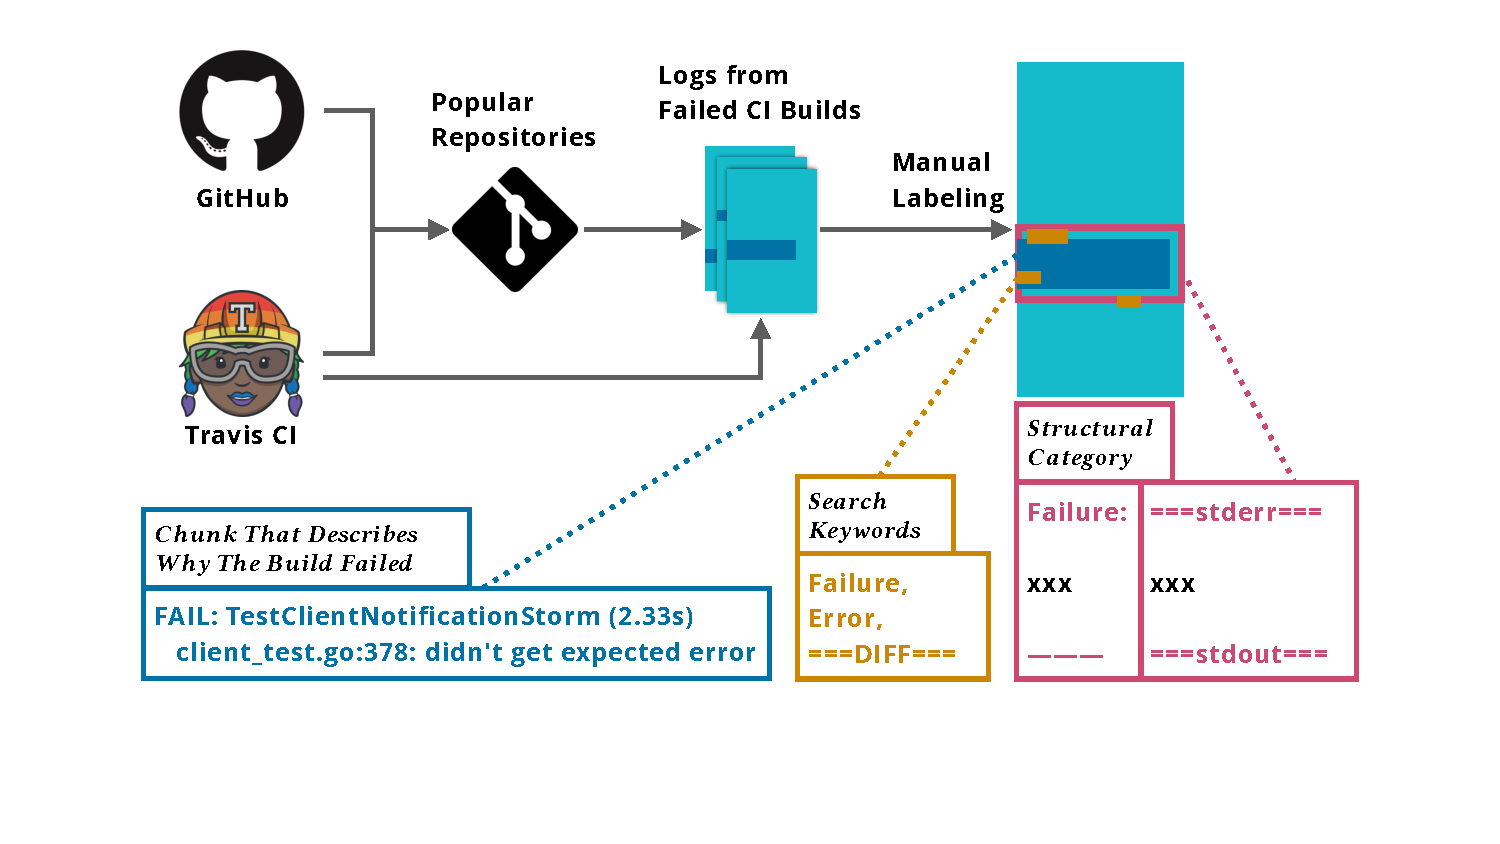
\includegraphics[width=\columnwidth, trim={2cm 2cm 2cm 0.5cm}, clip]{overview.pdf}
	\caption{Overview of \emph{LogChunks}}
	\label{fig:lc-overview}
\end{figure}

%\section{Applications}
%This section possible use cases for \emph{LogChunks} and outlines how we previously applied it to compare different build log analysis techniques.
\section{Potential Use Cases}

%\subsection{Potential Use Cases}
\emph{LogChunks} can be the basis for a wide range of further studies:

\paragraph{Benchmarking Build Log Analysis Techniques}
We created this data set to compare different techniques to retrieve chunks from build logs. %\todo{cite journal paper (or preprint?)}.
The techniques we compared are based on program synthesis from examples, text similarity and searching for keywords.
\emph{LogChunks} can be a benchmark to evaluate further build log analysis techniques.
For example, we can use the data set to investigate how reliable the diff and information retrieval approach of Amar et al.~\cite{amar2019mining} retrieves the reason a build failed.

\paragraph{Support Build Log Classification Algorithms}
Various researchers are looking into why CI builds fail and use build logs as a data source~\cite{seo2014programmers,vassallo2017a-tale}.
They write custom parsers and classifiers to categorize builds according to why a build failed.
The manually labeled chunk describing why the build failed can show classification algorithms where in a build log they can find information relevant for the classification.

\paragraph{Analysis of Keywords Used to Search for Build Failure Descriptions}
\emph{LogChunks} provides keywords that the authors would use to search for the chunk describing why the build failed.
Analyzing these can help us understand how users process build logs and which keywords a tool should use to mark an error description.
We can also recommend users which search keywords they should use to find why the build failed.

\paragraph{Studying Conversations about Build Failures}
Researchers are looking into conversations of developers surrounding CI builds and pull requests \todo{citation pending}
%TODO Caro: nathan cassee (with Alexander Sebrenik) did this in his master thesis (paper got accepted, will get link when preprint is finished), did not find others yet that do this}.
The chunks describing why a build failed, or the results of build log analysis techniques trained on them, can support these researchers to detect when a conversation participant is referring to the build failure described in the log.

% Andy also proposed: automatic creation of issue reports on GitHub with extracted info: sounds okay, but build failures are to be fixed faster than a GH issue I would say 

% \subsection{Chunk Retrieval Evaluation}
% We created \emph{LogChunks} to evaluate and compare different chunk retrieval techniques for build logs.
% The first technique is based on synthesizing programs from examples using the Microsoft PROSE library.
% A user provides a small number of examples to describe which text part the program should extract.
% PROSE then synthesizes a program of regular expressions that is consistent with these examples.
% We compared this extraction technique to a text similarity approach, which selects the lines of a build log which are most similar to the ones in the given user examples.
% Lastly, we investigated searching for keywords that are associated with the given user examples.

% The log chunks in this data set provided the examples for these techniques, the keywords were used to configure the keyword search.
% The structural categories enabled us to measure how structurally similar the examples have to be for a technique to be applicable.

% Our results show that program synthesis is well suited to retrieve information chunks from build logs when the targeted information is always presented in a structurally identical way and the user requires a high confidence in the precision and recall of the output.
% Using text similarity is advisable when precision is valued higher than recall and we recommend keyword search when recall is valued higher than precision.
% We present more detailed results, background and our study design in \todo{ref (preprint or so?) of full journal paper (or thesis?)}.

\section{Related Data Sets}
\label{sec:related-data-sets}
This section presents existing data sets of CI build logs and why \emph{LogChunks} is unique among them.

\subsection{TravisTorrent}
The \emph{TravisTorrent} data set~\cite{beller2017travistorrent} collects a broad range of metadata about builds on Travis CI\@.
It combines data accessible through the public Travis CI API~\cite{travisci2019apidoc} and related data from GitHub~\cite{github2019website} through GHTorrent~\cite{gousios2013ghtorrent}. They provide the names of failing test cases.
However, they obtained these through a manually developed parser, which only supports specific Ruby test runners and Java Maven or JUnit logs.
\emph{LogChunks} provides manually labeled data on the description of why builds failed for a much wider selection of build tools.

\subsection{Travis CI Build Log Data Set}
Loriot et al.~\cite{loriot2019dataset, loriot2019styler} collected Travis CI build logs from 130 GitHub repositories to analyze their use of the Checkstyle plugin.
They selected Maven repositories that included the Checkstyle plugin.
Their data set only provides the plain build logs, whereas \emph{LogChunks} additionally provides manually labeled data about the chunk describing why a build failed.

\section{Data Schema}
\label{sec:data-schema}

This section presents the file structure and the data schema of \emph{LogChunks}.
%We give a description of the manually labeled data.
%\emph{LogChunks} has two top level folders, \texttt{build-failure-reason} and \texttt{logs}.
%Each contains folders representing the main languages of the repositories in \emph{LogChunks}.
The build logs are organized in folders for each language and repository.
Within each repository folder, folders for each build status contain the log files named with the corresponding build ID.
% the logs are separated according to build status.
%Currently, \emph{LogChunks} only contains logs from \texttt{failed} builds.
%The build status folder contains the full logs in files named with the ID of the build that produced the log.

The folder \texttt{build-failure-reason} contains the manually labeled data of \emph{LogChunks}.
The data set provides an XML file for each repository: \texttt{\textless repository\_owner\textgreater @\textless repository\_name\textgreater.xml}.
Listing~\ref{lst:examples} presents the schema of these XML files.

For each repository, \emph{LogChunks} gives about 10 \texttt{Examples}.
Figure \ref{tab:data-in-example} presents the data within each example.
% Each \texttt{Example} consists of:
% \begin{itemize}
% 	\item \texttt{Log:} the relative path to the input build log.
% 	\item \texttt{Chunk:} the log chunk that describes why the build failed.
% 	\item \texttt{Keywords:} keywords the authors would use to search for the log chunk.
% 	\item \texttt{Category:} a categorization of the structural representation of the log chunk within the build log.
% 				The category is relative to the other examples for the same repository.
% \end{itemize}
Following, this section defines in more detail the labeled log chunk, search keywords and structural categories.

\lstset{
  language=XML,
  morekeywords={Examples, Example, Log, Keywords, Category, Chunk},
  postbreak=\mbox{\textcolor{cyan}{$\hookrightarrow$}\space},
	frame=single,
	escapeinside=**
}
\begin{figure}[]
	\centering
\begin{lstlisting}[breaklines=true]
<Examples>
  <Log>C/php@php-src/failed/529279089.log</Log>
    <Keywords>ERROR, FAIL, DIFF</Keywords>
    <Category>0</Category>
    <Chunk>001+ ** ERROR: process timed out **
001- OK.
========DONE========
FAIL Bug #60120 (proc_open hangs)</Chunk>
  </Example>
  ...
</Examples>
\end{lstlisting}
	\caption{Example XML file from \emph{LogChunks}}
	\label{lst:examples}
\end{figure}


\begin{figure*}[htbp]
\centering
\begin{tabularx}{\textwidth}{@{}lXlX@{}}
  \toprule
  & Description & Unit & Example \\
  \midrule
  Log & relative path to the input build log & Path to Log File & Haskell/koalaman@shellcheck/failed/501296412.log \\
  Chunk & log chunk that describes why the build failed & String & shellcheck.hs:442:19: error:
    Variable not in scope: doesPathExist :: [Char] -> IO Bool \\ 
  Keywords & keywords the authors would use to search for the log chunk & Strings & Failures, FAILURE, FAILED \\ 
  Category & categorization of the structural representation of the log chunk within the build log & Integer & 0 \\
  \bottomrule
\end{tabularx}
\caption{Data within an example in \emph{LogChunks}}
\label{tab:data-in-example}
\end{figure*}

\paragraph{Chunk That Describes Why The Build Failed}
The \texttt{Chunk} is the substring of the build logs that describes why the build failed.
This can, for example, be the failing test case or a compiler error and is one continuous substring of the build log.
When the reason \emph{why} the build failed was described in an external log, the \texttt{Chunk} includes the description \emph{that} the build failed.
%Wherever possible, it does \emph{not} include the log statements describing \emph{that} the build failed, but the description of \emph{why} it failed.
%For a few logs we were unable to define the section detailing why the build failed, e.g.\ because this information was logged in another log file.
%In these instances the \texttt{Chunk} contains the lines describing that the build failed.

\paragraph{Keywords}
The \texttt{Keywords} contain a list of one to three keywords appearing within the \texttt{Chunk} or in the area around it in the build log.
We selected keywords the authors would use to search for the log \texttt{Chunk} after analyzing about 800 build logs manually.
Some keywords from \emph{LogChunks} are: ``\texttt{FAIL}'', ``\texttt{Error}'', ``\texttt{=DIFF=}'' or ``\texttt{ERR!}''.

\paragraph{Category}
For each repository, we assign \emph{structural categories} to the chunks.
The structural category compares how \texttt{Chunk}s are represented within the build log.
Build tools highlight their error messages with markings, e.g.\ starting each line with ``\texttt{ERROR}'' or surrounding special characters.
Two chunks fall into the same structural categories if they are surrounded by the same markings.
Listing \ref{lst:same-category} presents a log chunk from the same category as the log chunk from Listing \ref{lst:examples}.
In comparison to that, Listing \ref{lst:different-category} presents a log chunk which is formatted differently within the log file.
%For most cases, two \texttt{Chunk} examples that fall into one category are outputted either within the same build phase or by the same build tool.
For each repository, the structural categories are represented as integers, starting at 0 and increased with the next appearing category in chronological build order.

\begin{figure}[tbp]
	\centering
\begin{lstlisting}[breaklines=true]
========DIFF========
*{\color{cyan}-=-=-=-=-=-}*
005+     Parameter #1 [<optional> $flags]
005-     Parameter #1 [<optional> $ar_flags]
========DONE========
FAIL Bug#71412 ArrayIterator reflection 
*{\color{cyan}-=-=-=-=-=-}*
TEST 9895/13942 [2/2 test workers running]
\end{lstlisting}
	\caption{Log chunk from the \emph{same} structural category than the log chunk presented in Listing \ref{lst:examples}, ``{\color{cyan}-=-=-=-=-=-}'' separates the log chunk from the context}
	\label{lst:same-category}
\end{figure}

\begin{figure}[tbp]
	\centering
\begin{lstlisting}[breaklines=true]
[0K$ ./sapi/cli/php run-tests.php -P ...
*{\color{cyan}-=-=-=-=-=-}*
Illegal switch 'j' specified!
*{\color{cyan}-=-=-=-=-=-}*
Synopsis:
\end{lstlisting}
	\caption{Log chunk from a \emph{different} structural category than the log chunk presented in Listing \ref{lst:examples}}
  %, ``{\color{cyan}-=-=-=-=-=-}'' separates the log chunk from the context}
	\label{lst:different-category}
\end{figure}

\section{Data Collection Process}
This section presents how we gathered the logs for \emph{LogChunks} and our manual labeling process.
\label{sec:data-collection}

\subsection{Log Collection}
We describe how we select the repositories, builds and logs for \emph{LogChunks}.
To collect the build logs we built the  \texttt{GHTorrentParser} and \texttt{TravisRequester} using Ruby.

\paragraph{Repository Sampling}
%First, we determine a set of repositories to query logs from.
Our \texttt{GHTorrentParser} queries the \emph{GHTorrent}~\cite{gousios2013ghtorrent} data set for the most popular languages on GitHub.
It then retrieves the most popular repositories for a given language.
We define \emph{Popularity} as the number of watches.
The \texttt{TravisRequester}, our tool querying the Travis API~\cite{travisci2019apidoc}, then checks whether a given repository uses Travis CI\@.

For \emph{LogChunks} we queried GHTorrent on 01/04/2018 for the three most popular repositories of each of the 30 most popular languages.
Among the resulting repositories are, for example, \texttt{git/git},  \texttt{Microsoft/TypeScript} and \texttt{jwilm/alacritty}.

\paragraph{Build Sampling}
The \texttt{TravisRequester} obtains the newest builds for a given repository.
We use a stratified sampling approach and save the obtained builds in buckets according to their status.
%We encountered the following statuses during our data collection: created, started, cancelled, passed, errored and failed.
The user of \texttt{TravisRequester} configures how many builds should be checked and how many builds per status should be saved.

To sample the builds for \emph{LogChunks} we let \texttt{TravisRequester} check up to 1000 builds per repository and keep ten of the status \emph{failed}~\cite{travis2009buildstatus}.
%A Travis CI build is marked as \emph{failed} when it faults in the \texttt{script} section of the build configuration defined by the user.

\paragraph{Log Sampling}
For each build, the \texttt{TravisRequester} then selects a log to download.
Travis CI links logs to \emph{jobs}.
A build can consist of multiple jobs, e.g.\ executing tests in different environments.
%A failed build can have successful job executions, as just one failed job leads to the whole build being marked as failed.
\texttt{TravisRequester} queries each build for the first job which has the same state and obtains the corresponding build log.

We inspected the collected build logs and discarded logs from three repositories.
One had only one failed build, two others had empty build logs on Travis CI\@.
In total we collected 797 logs from 80 repositories spanning 29 languages.

\subsection{Labeling Process}
\label{sec:labeling-process}
After collecting a wide range of Travis CI build logs we manually labeled which text chunk describes why the build failed.
Following that, we assigned search keywords and structural categories to each log chunk.

\paragraph{Chunk That Describes Why The Build Failed}
For each repository, the labeler skimmed through the build logs and copied out the first occurrence of a description why the build failed.
%They copied out the first continuous description as the \texttt{Chunk}.
They preserved whitespace and special characters, as they might be crucial to detect the targeted substring.
To support learning of regular expressions identifying the labeled substrings the labeler aimed to start and end the labeled substring at consistent locations around the fault description.

\paragraph{Keywords}
We presented the \texttt{Chunk} and ten lines above and below to the labeler.
Their task was to note down three strings they would put into a search field to find this failure description.
The strings should appear in or around the \texttt{Chunk} and is case-sensitive.
There are no limitations on the search string, especially spaces are allowed.

\paragraph{Category}
To label the \emph{structural categories} we presented the \texttt{Chunk} and the surrounding context to the labeler for all logs from a repository.
We asked them to assign numerical categories according to whether the \texttt{Chunk} had the same structural representation.
%The labeler should start the categories with 0 and increase as new ones appear.
%For reproducibility, we presented the logs in chronological build order.


\section{Data Set Validation}
\label{sec:validation}
% We validate our collected data points in two different ways.
% A different labeler performed a second pass of labeling the build failure reason, keywords and structural categories on a subset of the data.
% In addition, we sent out a survey to the developers, whose commits triggered the builds within our data set.
% We asked them whether our retrieval of the log part describing the reason the build failed was correct.
%This sections describes these two validation studies.
Following we present the two studies we conduct to validate the labeled data in \emph{LogChunks}.

\subsection{Inter-Rater Reliability Study}
To evaluate the validity of our labeled data points we perform a second labeling of a sample of the data in \emph{LogChunks}.

\paragraph{Method}
We followed the same labeling process as described in Section~\ref{sec:labeling-process}.
For the build failure reason and the keywords, we presented 30 randomly sampled build logs from distinct repositories in \emph{LogChunks}.
The structural categories are relative to other logs from the same repository.
Therefore, we randomly sampled 3 repositories and presented all 10 examples within them to the second labeler.

\paragraph{Results}
For the substring describing why the build failed, the two labelers exactly agreed in six cases.
In 15 cases the second labeler selected more lines, in five their selections overlapped and in four they completely disagreed.
Regarding the keywords, the two labelers completely agreed in nine cases and completely disagreed in two cases.
In nineteen cases there was  overlap in the keywords of the two labelers.%, in two the first labeler selected additional keywords compared to the second, while the second labeler proposed additional keywords in seven cases.
When classifying the chunks into structural categories, the two labelers agreed in 26 cases and disagreed in four cases.

% TODO Moritz: this is to answer questions 'why did you not do this standard thing': maybe there is a better position and/or way of saying this?
We found that calculating the standard measure for inter-rater agreement, Cohen's Kappa, is not applicable here.
For the log chunk it cannot represent the impact of overlapping selections of the labelers and for the keywords and structural categories the values the labelers could assign were not fixed.

\paragraph{Discussion}
The results of this validation study show that there is overlap in the data from both labelers, however also a high variation.
We believe that the main cause for this is that our explanations to the second labeler were not extensive enough.
There were implicit, inconsistent assumptions both labelers created during their work.
% In the following we describe these assumptions from both labelers for each data point and the implications on our description of the data classes.

% For the first data class, the reason the build failed, it was ambiguous whether the labeled substring should contain the information \emph{that} the build failed.
% This concerns statements like ``\texttt{The build exited with 1}''.
% One labeler included such statements, while the other one only focussed on the log parts describing \emph{why} the build failed, e.g.\ the name of the failing test case.

% While labeling the keywords a developer would use to search for the log part describing why the build failed, the one labeler allowed arbitrary strings appearing around the presented log part.
% In contrast to that, the other labeler focussed on actual \emph{words}, delimited by spaces or special characters.
% One labeler ignored capitalization, while the other one selected case-sensitive keywords.
% A third difference was that the first labeler was presented with all substrings from a repository, yielding more general keywords than the second labeler.

% For the structural categories this validation study showed a high overlap.
% In our instructions to the second labeler we did not emphasize the \emph{structural} aspect enough.
% They sorted into categories along \emph{why} the build failed, putting failing tests from different test runners into the same category even though the failing tests were presented differently in the log.
%
Our main learning from this study is that it is important and difficult to adequately communicate all decisions and assumptions on how data is labeled.
We reviewed the misunderstandings and incorporated more thorough descriptions in Section~\ref{sec:data-schema}.


\subsection{Developer Survey}
%For \emph{LogChunks} we analyzed around 800 build logs from different repositories and tried to extract the part of the log which describes why the respective build failed.
%As we are not involved in the development of any of the projects within our data set we could only rely on our previous experience with various build logs and systems.
%We only took the logs into account and did not check the related configurations, so it is well possible that we extracted parts that do describe errors but the respective step failing is ignored by the configuration and the build failed for another reason.
%
%The person who probably knows best why a build failed is the one committing the changes which triggered the build.
%If the build was e.g.\ part of a pull request then developer likely inspected the failed build and tried to fix the build so the pull request can be accepted.
We sent out mails to the original developers whose commits triggered the builds represented in \emph{LogChunks} and asked them whether the log chunk we labeled actually describes why the build failed.
This section describes our survey and discusses our results.

\paragraph{Method}
Using the Travis API, we collect the commit information for each build represented in \emph{LogChunks}.
We grouped all commits triggered by one developer and sent out an mail to them.%, asking whether the log part selected during our labeling was indeed describing the reason the build failed.
%Figure~\ref{fig:dev-mail} shows one of the mails sent out.
The mail included links to the corresponding commits, build overview and log file.
We asked the receivers to fill out a short survey in case our extraction was not correct.
%Look at Figure~\ref{fig:dev-survey} to get an impression of the survey.
In the survey, we asked the developer to paste in the log part actually describing the failure reason or describe why we were wrong in their own words.
As some of the chunks we labeled are many lines long, we trimmed all down to 10 lines to keep the mail readable.

\paragraph{Results}
In total we sent out mails to 246 developers.%, asking about 3.2 build logs per mail on average.
32 of these mails could not be delivered, e.g.\ because they were addressed to \emph{noreply} addresses.
%These 32 mails related to 68 of the build logs.
We received answers from 61 developers, corresponding with 144 build logs.
%Figure~\ref{fig:mails-answers-received-mails} and Figure~\ref{fig:mails-answers-received-builds} show the proportions of mails and logs answered about, not delivered and unanswered.

Of the 144 answers, 132 said our extraction was correct.
%26 answered either ``close, but not quite correct'' or ``no, the build failed for another reason''.
We manually inspected the 26 negative answers and found that some stated that the proposed extraction did not show the whole description of why the build failed.
This is because we had to trim long chunks to keep the mails readable.
After adjusting these answers, 12 answers stated that our labeled log chunk was not correct.

\paragraph{Discussion}
This study highly strengthens the trust in the validity of the labeled log chunks.
The study received answers about 18\% of the logs from \emph{LogChunks}.
After manual correction, 91\% of the received answers said our labeled chunks were accurate.

One of our extractions only showed a warning and the developer proposed to also include the line stating that warnings are treated as errors.
In others that were identified as incorrect, we labeled the error message of an error that was later ignored.

\section{Summary}
\label{sec:conclusion}
In this paper, we introduced the \emph{LogChunks} data set encompassing 797 build logs from 80 projects using Travis CI\@.
For each log, we annotated the log chunk describing why the build failed and provide keywords a developer would use to search for the log chunk as well as a categorization of the log chunks according to their format within the log.

\emph{LogChunks} advances the research field of build log analysis by introducing a benchmark to rigorously examine research contributions~\cite{sim2003using}.

Still, there are limitations to our data set, which we present in the following, together with improvements and extensions to \emph{LogChunks}.

\paragraph{Chunk as One Consecutive Substring}
The manually labeled \texttt{Chunk} contains only one continuous substring of the log text.
The reason a build failed could be described at multiple locations within the log.
We propose to extend \emph{LogChunks} to contain multiple substrings of the log text.

\paragraph{Include More Repositories and Logs}
\emph{LogChunks} encompasses a wide range of repositories from various main development languages, though only 10 logs from each repository.
%This stems from the high effort necessary for the manual data labeling process.
Including more logs and repositories into \emph{LogChunks} will strengthen it as a benchmark to compare build log analysis techniques.

\paragraph{Classification of the Build Failure Cause}
Our data set contains no further classification according to the cause of the failure.
As researchers are investigating why CI builds fail, a useful extension is to annotate cause of the build failure for each log.

\paragraph{Other Targeted Information Chunks}
Build log analysis is not limited to retrieving the chunk describing why a build failed.
\emph{LogChunks} can be extended with further information targets such as descriptions of warnings, build infrastructure and more.

\paragraph{Validation of Search Keywords}
The keywords \emph{LogChunks} provides are based on the experience of the authors gained from analyzing around 800 build logs.
Next, we propose to evaluate whether these keywords would also be used by developers to find the log chunk describing why a build failed.

%%
%% The acknowledgments section is defined using the "acks" environment
%% (and NOT an unnumbered section). This ensures the proper
%% identification of the section in the article metadata, and the
%% consistent spelling of the heading.

% \begin{acks}
% To Robert, for the bagels and explaining CMYK and color spaces.
% \end{acks}

%%
%% The next two lines define the bibliography style to be used, and
%% the bibliography file.
\bibliographystyle{ACM-Reference-Format}
\bibliography{paper}

%%
%% If your work has an appendix, this is the place to put it.
% \appendix

% \section{Research Methods}

% \subsection{Part One}


\end{document}
\endinput
%%
%% End of file `sample-sigconf.tex'.
